\documentclass[12pt]{article}

\usepackage{sbc-template}
\usepackage[brazil,american]{babel}
\usepackage[utf8]{inputenc}

\usepackage{graphicx}
\usepackage{url}
\usepackage{float}
\usepackage{listings}
\usepackage{color}
\usepackage{todonotes}
\usepackage{algorithmic}
\usepackage{algorithm}
\usepackage{hyperref}
\usepackage{indentfirst}
\usepackage[inline]{enumitem}


\graphicspath{{./images/}}

\sloppy

\title{Laboratório 3\\- CPU MIPS Uniciclo –}

\author{GRUPO 6\\
	Dayanne Fernandes da Cunha, 13/0107191\\
	Lucas Mafra Chagas, 12/0126443\\
	Marcelo Giordano Martins Costa de Oliveira, 12/0037301\\
	Lucas Junior Ribas, 16/0052289\\
	Caio Nunes de Alencar Osório, 16/0115132\\
	Diego Vaz Fernandes, 16/0117925}

\address{Dep. Ciência da Computação -- Universidade de Brasília (UnB)\\
  CiC 116394 - OAC - Turma A
  \email{}
}

\begin{document}
\maketitle

\section{Objetivos}
\label{sec:Objetivos}

\begin{itemize}
\item Treinar o aluno com a linguagem de descrição de \textit{hardware} \textit{Verilog};
\item Familiarizar o aluno com a plataforma de desenvolvimento \textit{FPGA DE2} da \textit{Altera} e o software \textit{QUARTUS II};
\item Desenvolver a capacidade de análise e síntese de sistemas digitais usando uma Linguagem de Descrição de \textit{Hardware};
\item Apresentar ao aluno a implementação de uma \textit{CPU MIPS}.
\end{itemize}

\section{Ferramentas}
\label{sec:Materiais}

Todos os códigos escritos neste laboratório podem ser encontrados no repositório \url{https://github.com/Dayof/OAC172} do \textit{GitHub}.

\begin{itemize}
\item FPGA DE2 da Altera 
\item QUARTUS-II
\item Verilog HDL
\end{itemize}

\section{Exercícios - PARTE A}
\label{sec:exerciciosA}

\subsection{Exercício 4. Diagrama de fluxo para tratamento de exceção}
\label{subsec:dfluxoexc}

%\begin{figure}[H]
%	\centering
%	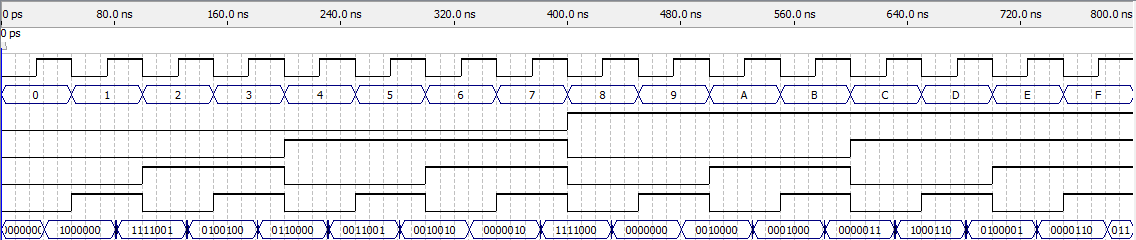
\includegraphics[width=.8\textwidth]{ex1_st.png}
%	\caption{Simulação síncrona temporal do \textit{decoder7}.}
%	\label{fig:ex1st}
%\end{figure}

\subsection{Exercício 5. Software de lançamento de bola de canhão na FPGA}
\label{subsec:canhao}

\section{Exercícios - PARTE B}
\label{sec:exerciciosB}

\subsection{Exercício 7. Processador \textit{MIPS PUMv.5.0} UNICICLO}
\label{subsec:mips_uniciclo}

\subsection{Exercício 8. Teste do funcionamento das instruções da \textit{ISA}}
\label{subsec:testeisa}
 
\subsection{Exercício 9. Novas instruções usando a \textit{ISA MIPS}}
\label{subsec:newint}

\bibliographystyle{sbc}
\bibliography{relatorio}

\end{document}
